% Variational autoencoder architecture. The earliest type of generative machine learning model.
% Inspired by https://towardsdatascience.com/intuitively-understanding-variational-autoencoders-1bfe67eb5daf.

\documentclass[tikz]{standalone}

\usepackage{xstring}

\usetikzlibrary{fit,positioning}

\newcommand\drawNodes[2]{
  % #1 (str): namespace
  % #2 (list[list[str]]): list of labels to print in the node of each neuron
  \foreach \neurons [count=\lyrIdx] in #2 {
    \StrCount{\neurons}{,}[\lyrLength] % use xstring package to save each layer size into \lyrLength macro
    \foreach \n [count=\nIdx] in \neurons
      \node[neuron] (#1-\lyrIdx-\nIdx) at (2*\lyrIdx, \lyrLength/2-1.4*\nIdx) {\n};
  }
}

\newcommand\denselyConnectNodes[2]{
  % #1 (str): namespace
  % #2 (list[int]): number of nodes in each layer
  \foreach \n [count=\lyrIdx, remember=\lyrIdx as \previdx, remember=\n as \prevn] in #2 {
    \foreach \y in {1,...,\n} {
      \ifnum \lyrIdx > 1
        \foreach \x in {1,...,\prevn}
          \draw[->] (#1-\previdx-\x) -- (#1-\lyrIdx-\y);
      \fi
    }
  }
}

\begin{document}
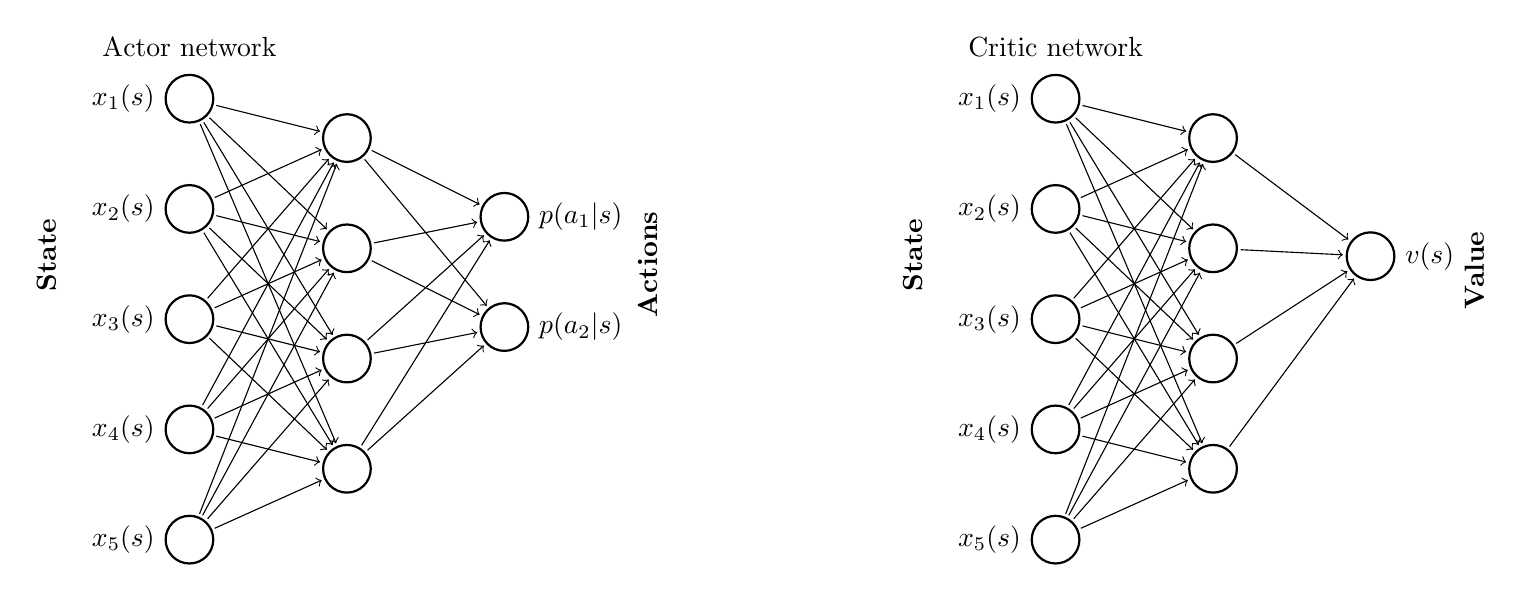
\begin{tikzpicture}[
    shorten >=1pt, shorten <=1pt,
    neuron/.style={circle, draw, minimum size=4ex, thick},
    legend/.style={font=\large\bfseries},
  ]

  % actor
  \drawNodes{actor}{{{,,,,}, {,,,}, {,}}}
  \denselyConnectNodes{actor}{{5, 4, 2}}

  % input + output labels
  \foreach \idx in {1,...,5} {
      \node[left=0 of actor-1-\idx] {$x_\idx(s)$};
    }
  \foreach \idx in {1,...,2} {
      \node[right=0 of actor-3-\idx] {$p(a_\idx|s)$};
    }

  \node[above=0.1 of actor-1-1] {Actor network};
  \node[left=1.5 of actor-1-2, rotate=90] {\textbf{State}};
  \node[right=1.5 of actor-3-2, rotate=90] {\textbf{Actions}};

  % critic
  \begin{scope}[xshift=11cm]
    \drawNodes{critic}{{{,,,,}, {,,,}, {\\}}}
  \denselyConnectNodes{critic}{{5, 4, 1}}
  \end{scope}
  % input + output labels
  \foreach \idx in {1,...,5} {
      \node[left=0 of critic-1-\idx] {$x_\idx(s)$};
    }
  \node[right=0 of critic-3-1] {$v(s)$};
  \node[above=0.1 of critic-1-1] {Critic network};
  \node[left=1.5 of critic-1-2, rotate=90] {\textbf{State}};
  \node[right=5 of critic-1-3, rotate=90] {\textbf{Value}};

\end{tikzpicture}
\end{document}